En esta sección vamos a demostrar el potencial de la herramienta con algunos ejemplos de su funcionamiento. Validando el funcionamiento de ésta, y sus mejoras funcionales con respecto a la versión de Scratch4Robots de la que partimos.\\

Además de los ejemplos mostrados en este apartado, se ha creado una batería de pruebas con las que ver un ejemplo de funcionamiento de cada uno de nuestros bloques. Estas pruebas son proyectos Scratch, que el usuario puede cargar en el entorno de Scratch y usar como punto de partida para sus próximos proyectos.

\section{Evitar obstáculos con Turtlebot}
\label{sec:evitar-obstaculos}

En este ejemplo hacemos uso de un robot con ruedas, para ser más exactos de un Turtlebot. Para ejecutar las pruebas utilizamos Gazebo como simulador, cargando un entorno con obstáculos repartidos como se aprecia en la figura.\\

El objetivo directo de este experimento es la programación de un robot Turtlebot, capaz de evitar obstáculos de forma autónoma, con la ayuda de un sensor láser incorporado en su parte frontal. Esto lo vamos a conseguir usando únicamente la lógica de la que disponemos en Scratch junto con la extensión que aporta nuestra aplicación Scratch4Robots.\\

Se puede apreciar con estos ejemplos el poder didáctico de la herramienta. Su simpleza y sencillez hacen de ella perfecta para la enseñanza a personas con pocos conocimientos técnicos.

Además este ejemplo podemos verlo en nuestro día a día con las famosas aspiradoras autónomas (iRobot Roomba), por lo que vemos una aplicación directa que podría tener nuestra aplicación fuera del ámbito didáctico.

Vamos a seguir el ciclo de vida de nuestra aplicación, explicando el proceso que lleva a la consecución de nuestro objetivo.

En primer lugar y con ayuda de nuestros bloques, desarrollamos la aplicación en Scratch. Una vez tenemos nuestro proyecto acabado y guardado, con la herramienta Scratch4Robots, ya instalada en nuestro equipo y mediante el uso de un solo comando realizaremos la traducción del proyecto.\\

\begin{figure}[H]
    \centering
    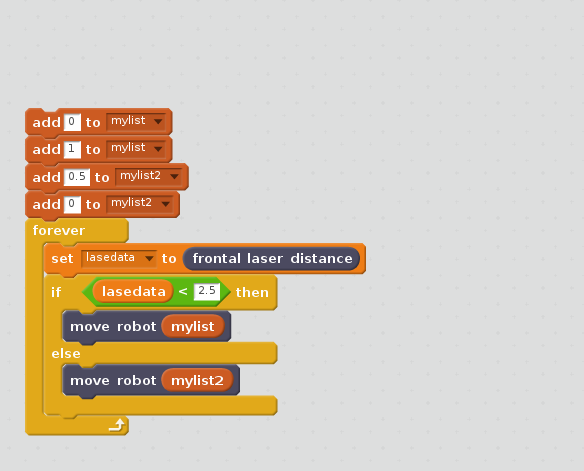
\includegraphics[scale=0.60]{img/robot-obstaculos-scratch.PNG}
  	\caption{Programación en Scratch del Turtlebot}
  	\label{fig:turtlebot}
\end{figure}

Esta simpleza en la ejecución la conseguimos mediante las funcionalidades que nos aporta ROS para la ejecución de nodos, esto se consigue tras la labor de integración realizada. El comando a ejecutar sería:
\pagebreak

\begin{lstlisting}[language=json,firstnumber=1]
~$ rosrun scratch4robots scratch2python myscratchaproyect.sb2
\end{lstlisting}


Explicando un poco el comando anterior, \textit{rosrun} sería el comando que nos aporta ROS, capaz de ejecutar nodos de un paquete ROS, \textit{scratch4robots} es nuestro paquete ya instalado en la máquina, \textit{scratch2python} sería el nodo interno de nuestra aplicación encargada de la traducción a Python, y por último se añade el proyecto Scratch que queremos traducir. Observamos a continuación el código ya traducido a Python que será incrustado en el nodo ROS para su ejecución.

\begin{lstlisting}[language=python,firstnumber=1]
        mylist = []
        mylist2 = []
		# Agrega velocidades que realizan el giro del Turtlebot
        mylist.append('0')
        mylist.append('1')
        # Agrega velocidades que hacen que el Turtlebot avance
        mylist2.append('0.5')
        mylist2.append('0')
        while True:
            lasedata = robot.get_laser_distance()
            if lasedata < 2.5:
                robot.move_vector(mylist)
            else:
                robot.move_vector(mylist2)
                
\end{lstlisting}

Tras la traducción obtenemos un nodo ROS completamente preparado para su ejecución sobre el robot Turtlebot, únicamente con la dependencia de un fichero de configuración que describiremos a continuación:
\pagebreak
\begin{lstlisting}[language=json,firstnumber=1]
robot:
  Motors:
    Server: 2 # ROS
    Topic: "/mobile_base/commands/velocity"
    Name: robotMotors
    maxW: 0.7
    maxV: 4

  Laser:
    Server: 2 # ROS
    Topic: "/scan"
    Name: robotLaser

  Pose3D:
    Server: 2 # ROS
    Topic: "/odom"
    Name: robotPose3d

  Camera1:
    Server: 2 # ROS
    Format: RGB8
    Topic: "/cameraL/image_raw"
    Name: robotCamera1

  NodeName: robot
\end{lstlisting}
En este fichero se observa los distintos actuadores y sensores que necesitará nuestro nodo, además por cada sensor se define el Tópico al que nuestro nodo se subscribe para enviar y recoger los datos que necesitemos de nuestro robot. En este caso darle especial importancia a la obtención de los datos del sensor laser, protagonista de nuestro ejemplo.

Con todo esto preparado solo faltaría ejecutar nuestro nodo sobre la simulación para ver los resultados que podemos apreciar en el siguente detalle.

\begin{figure}[H]
    \centering
    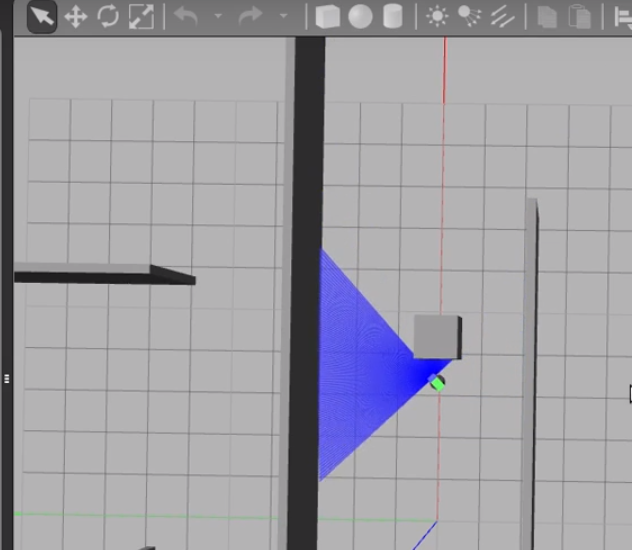
\includegraphics[scale=0.75]{img/robot-example.PNG}
  	\caption{Ejecución del nodo sobre Turtlebot}
  	\label{fig:turtlebot}
\end{figure}


De esta forma, en pocos y sencillos pasos conseguimos programar un robot de forma autónoma para que evite cualquier obstáculo que se encuentre en su camino.


\section{Persecución entre drones}
\label{sec:persecucion-drones}

En este ejemplo por el contrario, como robot final utilizamos un dron, mucho más interesante desde el punto de vista práctico, aunque igual de interesante desde el punto de vista didáctico. Al igual que con la prueba anterior hemos utilizado Gazebo como motor de simulación.\\

El ciclo de vida es el mismo que el que hemos seguido para la ejecución del robot. Primero se genera el proyecto en Scratch, el cual mostramos en la siguiente imagen:\\

\begin{figure}[H]
    \centering
    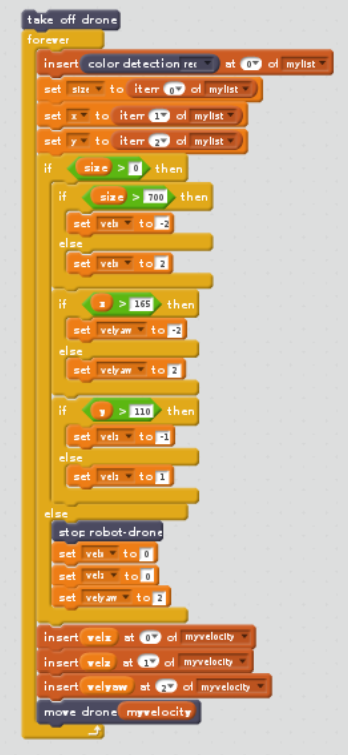
\includegraphics[scale=0.75]{img/cat-drone-scratch.PNG}
  	\caption{Programación en Scratch del drone perseguidor}
  	\label{fig:turtlebot}
\end{figure}

Mediante las funcionalidades que nos aporta ROS para el lanzamiento de aplicaciones bajo un solo comando ejecutamos la traducción, obteniendo nuestro nodo programado en Python. Mostramos el detalle de la traducción de este proyecto, la cual se integrará en el nodo final ROS como hemos descrito en apartados anteriores.

\begin{lstlisting}[language=python,firstnumber=1]
 		mylist = [] 
 		myvelocity = []
        robot.take_off()
        while True:
            mylist.insert(0, robot.color_detection('red'))
            size = mylist[0][0]
            x = mylist[0][1]
            y = mylist[0][2]
            if size > 0: 		 # Tras detectar el objetivo, estima velocidades
                if size > 700:
                    velx = '-2'
                else:
                    velx = '2'
                if x > 165:
                    velyaw = '-2'
                else:
                    velyaw = '2'               
                if y > 110:
                    velz = '-1'
                else:
                    velz = '1'               
            else:			# Gira sobre si mismo buscando el objetivo
                robot.stop()
                velx = '0'
                velz = '0'
                velyaw = '2'            
            myvelocity.insert(0, velx)
            myvelocity.insert(1, velz)
            myvelocity.insert(2, velyaw)
            robot.move_vector(myvelocity)
\end{lstlisting}

Y por último, ya con nuestro nodo generado, agregando la configuración pertinente estará todo listo para su ejecución.

\begin{lstlisting}[language=json,firstnumber=1]
drone:
  Camera:
    Format: RGB8
    Topic: "/solo/cam_frontal/image_raw"
    Name: UAVViewerCamera
    
  Pose3D:
    Topic: "/mavros/local_position/odom"
    Name: UAVViewerPose3d
    
  CMDVel:
    Topic: "/mavros/setpoint_velocity/cmd_vel"
    Name: UAVViewerCMDVel
    
  Navdata:
    Topic: "/IntrorobROS/Navdata"
    Name: UAVViewerNavdata
    
  Extra:
    TopicArming: "mavros/cmd/arming"
    TopicLand: "mavros/cmd/land"
    TopicSetMode: "mavros/set_mode"
    TopicVel: "/mavros/setpoint_velocity/cmd_vel"
    Name: UAVViewerExtra
NodeName: drone
\end{lstlisting}
Tras ejecutar el nodo junto con el fichero de configuración, obtenemos el resultado deseado, como observamos en la imagen superior. Algo tan complejo como una persecución entre dos drones, totalmente programado en un lenguaje tan simple como Scratch, y esto, es solo una prueba del potencial de esta herramienta.\\


\begin{figure}[H]
    \centering
    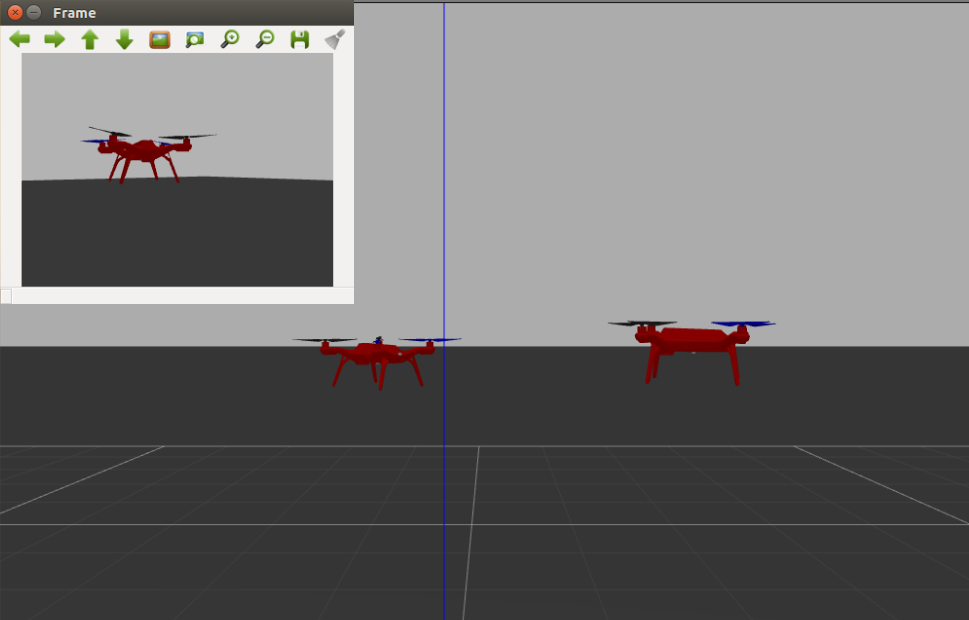
\includegraphics[scale=0.60]{img/drones-fly.PNG}
  	\caption{Ejecución del drone perseguidor}
  	\label{fig:drone-pers}
\end{figure}


Con estos ejemplos hemos recorrido el ciclo de vida de nuestra herramienta, explicando su funcionamiento, además de validar experimentalmente todas las mejoras en el funcionamiento de Scratch4Robots 2.0. Las mejoras en la ejecución de la herramienta mediante simples comandos, sin necesidad de indagar en el código fuente. Y completo funcionamiento de la herramienta, con comunicaciones ROS. 

